\documentclass[8pt]{extarticle}
\usepackage[a4paper,landscape,top=1.15cm,bottom=1.05cm,left=0.9cm,right=0.9cm,headsep=0.25cm,footskip=0.45cm]{geometry}
\usepackage{xeCJK}
\setCJKmainfont{Noto Serif CJK SC}[BoldFont={Noto Serif CJK SC Bold}]
\setCJKsansfont{Noto Sans CJK SC}
\setCJKmonofont{Noto Sans Mono CJK SC}
\setmonofont{DejaVu Sans Mono}[Scale=0.88]
\usepackage{amsmath,amssymb}
\usepackage[dvipsnames]{xcolor}
\usepackage{graphicx,multicol,booktabs,tabularx,array,enumitem,fancyhdr,needspace,fancyvrb,newunicodechar}
\usepackage[most]{tcolorbox}
\usepackage[hidelinks]{hyperref}

\newunicodechar{→}{\ensuremath{\rightarrow}}
\newunicodechar{←}{\ensuremath{\leftarrow}}
\newunicodechar{≥}{\ensuremath{\geq}}
\newunicodechar{≤}{\ensuremath{\leq}}
\newunicodechar{×}{\ensuremath{\times}}
\newunicodechar{≈}{\ensuremath{\approx}}
\newunicodechar{τ}{\ensuremath{\tau}}
\newunicodechar{−}{\ensuremath{-}}
\newunicodechar{⊂}{\ensuremath{\subset}}

\definecolor{cred}{HTML}{C0392B}\definecolor{cblue}{HTML}{2C3E9E}
\definecolor{cgreen}{HTML}{1E7A4C}\definecolor{cpurple}{HTML}{6C3483}
\definecolor{cteal}{HTML}{117A65}\definecolor{cgray}{HTML}{5D6D7E}
\definecolor{corange}{HTML}{B9770E}
\raggedcolumns\setlength{\columnsep}{11pt}\setlength{\columnseprule}{0.3pt}
\setlength{\parindent}{0pt}\setlength{\parskip}{1.5pt}
\linespread{1.0}
\setlist{nosep,leftmargin=1.0em,labelsep=0.3em}
\setlist[itemize]{label={\color{cgray}\textbullet}}
\newcolumntype{Y}{>{\raggedright\arraybackslash}X}
\setlength{\tabcolsep}{3pt}

\pagestyle{fancy}\fancyhf{}
\fancyhead[L]{\small LLM Agent 速查表 \#02}
\fancyhead[C]{\small\textsc{Cheatsheet: Test-Time Scaling}}
\fancyhead[R]{\small\texttt{2019 → 2026}}
\fancyfoot[L]{\small Prepared by Yiwen, with help from Claude}
\fancyfoot[C]{\small\thepage}\fancyfoot[R]{\small\textsc{Fall 2026}}
\renewcommand{\headrulewidth}{0.5pt}\renewcommand{\footrulewidth}{0.5pt}

\newcommand{\sect}[2][cred]{\par\vspace{4pt}{\color{#1}\rule[-2pt]{2.5pt}{10pt}}\hspace{3pt}{\large\bfseries\color{#1}#2}\par\nopagebreak\vspace{1pt}}
\newcommand{\sub}[1]{\par\vspace{2pt}{\bfseries\color{cteal}#1}\par\nopagebreak}
\newcommand{\paper}[2]{\par\vspace{3pt}{\bfseries\color{cblue}#1}\ {\scriptsize\color{cgray}#2}\par\nopagebreak}
\newcommand{\lab}[1]{{\bfseries\color{cred}#1}\,}
\newcommand{\ax}[1]{\href{https://arxiv.org/abs/#1}{\texttt{#1}}}
\newcommand{\note}[1]{\par{\itshape\color{cblue}#1}\par}

\newtcolorbox{tbox}[2][]{enhanced,colback=#2!5,colframe=#2!65,boxrule=0.5pt,arc=1.5pt,
  left=3pt,right=3pt,top=1.5pt,bottom=1.5pt,fonttitle=\bfseries\small,coltitle=black,colbacktitle=#2!16,
  toptitle=0.5pt,bottomtitle=0.5pt,before skip=3pt,after skip=3pt,#1}
\newenvironment{code}{\VerbatimEnvironment\begin{tcolorbox}[colback=gray!7,colframe=gray!45,boxrule=0.4pt,arc=1pt,left=2pt,right=2pt,top=0.5pt,bottom=0.5pt,before skip=2pt,after skip=2pt]\begin{Verbatim}[fontsize=\scriptsize]}{\end{Verbatim}\end{tcolorbox}}

\begin{document}
%==================== HEADER ====================
\begin{tcolorbox}[enhanced,colback=cblue!5,colframe=cblue!40,boxrule=0.6pt,arc=2pt,left=7pt,right=7pt,top=4pt,bottom=4pt]
\begin{minipage}[t]{0.56\linewidth}
{\fontsize{17}{21}\selectfont\bfseries Cheatsheet: Test-Time Scaling（2019 → 2026）}\par\vspace{2pt}
{\itshape\color{cgray} Parallel · Sequential · Search · Latent · Test-Time Training — how models spend compute at inference}\par
{\small\color{cgray} Yiwen 整理 · 90+ 篇论文与官方发布 · 数字均出自原文（arXiv / 官方博客）· 2026 年 10 月核对}
\end{minipage}\hfill
\begin{minipage}[t]{0.42\linewidth}\small
\textbf{核心问题：}模型训练完以后，\textbf{推理时多花算力}能不能换来更好的答案？花在哪里最划算？\\
\textbf{怎么读：}每节 \textbf{\color{cred}问题} → \textbf{\color{cblue}方法（算法 / 公式）} → \textbf{数字} → \textbf{\color{corange}局限}。\textbf{记号：}$x$ 题目，$y$ 解答，$\pi$ 生成模型，$V$ 验证器，$N$ 采样数，$C$ 推理算力预算。
\end{minipage}
\end{tcolorbox}

\begin{minipage}[t]{0.40\linewidth}\vspace{0pt}
\begin{tbox}[title={统一形式化：用推理算力换准确率}]{cblue}
\small
\textbf{Best-of-N}\ \ $y_i\sim\pi(\cdot|x),\ i=1..N$，\ $\hat y=\arg\max_{y_i}V(x,y_i)$\\
\textbf{多数投票}\ \ $\hat a=\arg\max_a\sum_i\mathbf{1}[\mathrm{ans}(y_i)=a]$\\
\textbf{加权投票}\ \ $\hat a=\arg\max_a\sum_i V(x,y_i)\,\mathbf{1}[\mathrm{ans}(y_i)=a]$\\
\textbf{覆盖率 pass@k}（无偏估计，$n$ 个样本中 $c$ 个对）：\\
\hspace*{1em}$\text{pass@}k=1-\binom{n-c}{k}\big/\binom{n}{k}$\\
\textbf{算力账}（Snell 等）：$X=\underbrace{6ND_{\text{pre}}}_{\text{预训练}}+\underbrace{2ND_{\text{inf}}}_{\text{推理}}$，$N$ 参数量，$D$ token 数\\
\textbf{Compute-optimal}：$\theta^*(x,C)=\arg\max_\theta\ \mathbb{E}_{y\sim\mathrm{Target}(\theta,C,x)}\big[\mathbf{1}[y=y^*]\big]$，按题目难度选策略 $\theta$\\[2pt]
\textbf{关键区分：}覆盖率需要\textbf{知道答案对不对}（oracle）；实际准确率受\textbf{挑选方法}（投票 / 验证器）限制。
\end{tbox}
\end{minipage}\hfill
\begin{minipage}[t]{0.585\linewidth}\vspace{0pt}
\begin{tbox}[title={五种花推理算力的方式}]{cgreen}
\small
\begin{tabularx}{\linewidth}{@{}p{1.15cm} p{2.9cm} p{4.4cm} Y@{}}
\toprule
方式 & 怎么花 & 代表 & 需要 / 局限\\\midrule
{\color{cblue}并行} & 独立采 $N$ 个再聚合 & Best-of-N、自一致性、Deep Think & 聚合器；投票会饱和\\
{\color{cblue}串行} & 一条写更长 / 反复修改 & CoT、Self-Refine、o1 / R1、s1 & 会自我纠错；想太多 / 太少\\
{\color{cblue}搜索} & 在中间步骤上展开、打分、剪枝 & ToT、PRM beam search、MCTS & 步骤级验证器；调用多\\
{\color{cblue}潜空间} & 循环更多层，不多写 token & Coconut、Recurrent Depth & 专门架构；不可读\\
{\color{cred}更新参数} & 在测试样本上训练 & TTT、TTT-ARC、TTRL、TTT-Discover & 自监督 / 伪标签；每题一次训练\\
\bottomrule
\end{tabularx}
\textbf{主线：}阶段 1–6 是\textbf{外挂}在模型外的算法 → 阶段 7 起被 \textbf{RL 训练进模型} → 2025 年后变成 \textbf{API 旋钮}（预算 / 强度 / 自适应）和\textbf{并行思考}顶配档。
\end{tbox}
\end{minipage}

\vspace{1pt}
\begin{multicols}{4}
%==================== 0 ====================
\sect{0. 前史：搜索可以替代训练（2021）}
\paper{Scaling Scaling Laws with Board Games}{Andy L. Jones · \ax{2104.03113} · 2021-04}
AlphaZero 下 Hex，同时改变训练算力和推理时 MCTS 算力：
\begin{tbox}[title=关键结论]{cgreen}\small
“训练算力每多 10×，大约可以省掉 15× 的推理算力”——两者在一条等性能线上可以互换（直到只剩单节点搜索）。
\end{tbox}
\note{语言模型缺两样东西：可以展开的搜索树，和可靠的打分函数。后面十年都在补这两样。}

%==================== 1 ====================
\sect{1. 多采几个，再挑一个（2021–2022）}
\paper{Training Verifiers (GSM8K)}{OpenAI · \ax{2110.14168} · 2021-10}
\begin{itemize}
\item GSM8K：8.5K 小学数学题（7.5K 训练 / 1K 测试）。
\item \textbf{验证器训练}：用生成器采的解，按最终答案对错打标签，训练模型预测“这个解对不对”（逐 token 预测价值）。
\item 推理：每题采 \textbf{100} 个解，取验证器分数最高的。
\item \textbf{6B + 验证器略胜微调的 175B}，相当于模型放大约 \textbf{30×}。
\item 采样数太大时效果反而下降：验证器会被“骗过”。
\end{itemize}
\paper{AlphaCode}{DeepMind · \ax{2203.07814} · 2022-02}
\begin{code}
每题采样 ~百万个程序
  → 用题目样例测试过滤（去掉约 99%）
  → 在生成的测试输入上按输出行为聚类
  → 每个大类挑一个，最多提交 10 个
\end{code}
Codeforces（5,000+ 人比赛）前 \textbf{54.3\%}，估计等级分 1238。
\begin{tbox}[title=局限]{corange}\small
需要单独训练验证器（或有可执行测试）；采样量大；验证器分数会被过度优化。
\end{tbox}

%==================== 2 ====================
\sect{2. 让模型多写几步：思维链（2022）}
\paper{Chain-of-Thought Prompting}{Google · \ax{2201.11903} · 2022-01}
\begin{itemize}
\item 少样本示例里写出推理过程。PaLM 540B GSM8K：17.9\% → \textbf{56.9\%}（超过当时微调 GPT-3 + 验证器的 55\%）。
\item 只有足够大的模型才受益（“涌现”）。
\end{itemize}
\paper{Zero-shot CoT}{东京大学 · \ax{2205.11916} · 2022-05}
\begin{code}
Q: ... A: Let's think step by step.
  → [推理]
Therefore, the answer (arabic numerals) is
  → [答案]
\end{code}
MultiArith 17.7 → 78.7，GSM8K 10.4 → 40.7（text-davinci-002）。
\note{要点：CoT 让每道题的计算量可变——难题可以写更多 token，这就是“串行”scaling 的起点。}

%==================== 3 ====================
\sect{3. 自一致性：多条推理投票（2022–2024）}
\paper{Self-Consistency}{Google · \ax{2203.11171} · 2022-03}
\begin{code}
for i in 1..N:   # 论文 N = 40，温度采样
    r_i, a_i ← sample CoT(x)
return majority_vote(a_1..a_N)  # 只看最终答案
\end{code}
{\small
\begin{tabularx}{\linewidth}{@{}Y r@{}}
\toprule
相对 CoT 贪心解码 & 提升\\\midrule
GSM8K / SVAMP / AQuA & +17.9 / +11.0 / +12.2\\
StrategyQA / ARC-c & +6.4 / +3.9\\
code-davinci-002 GSM8K & 60.1 → 78.0\\
PaLM-540B GSM8K & 56.5 → 74.4\\
\bottomrule
\end{tabularx}}
直觉：错误的推理五花八门，正确的推理殊途同归。
\paper{Universal Self-Consistency}{Google · \ax{2311.17311} · 2023-11}
开放式输出无法精确比对 → 把所有候选拼进提示，让模型选“最一致”的。PaLM 2-L GSM8K：贪心 85.7 / SC 90.4 / USC 90.2。
\paper{Are More LLM Calls All You Need?}{Stanford · \ax{2403.02419} · 2024-03}
投票准确率随调用次数可能\textbf{先升后降}：简单题越投越对，难题上错误答案占多数时越投越错。可以拟合出最优调用数 $K^*$。
\begin{tbox}[title=局限]{corange}\small
只看最终答案；需要答案可比对；会饱和（数百个样本后几乎不再涨）。
\end{tbox}

%==================== 4 ====================
\sect{4. 过程奖励：给每一步打分（2022–2024）}
\begin{tbox}[title=问题]{cred}\small
答案对，过程可能错；结果奖励（ORM）只看结尾，没法在推理中途指导搜索。
\end{tbox}
\paper{Process vs. Outcome Feedback}{DeepMind · \ax{2211.14275} · 2022-11}
GSM8K：两种监督最终答案错误率相近，但在答案正确的解中，\textbf{推理过程错误率 14.0\% → 3.4\%}（过程监督）。
\paper{Let's Verify Step by Step}{OpenAI · \ax{2305.20050} · 2023-05}
\begin{itemize}
\item \textbf{PRM800K}：人工给每一步标 正确 / 错误 / 中性，共 80 万个步骤标签；用主动学习专挑“答案错但看起来很像对的”解来标。
\item 整条解的分数 = 各步都正确的概率：$\mathrm{PRM}(y)=\prod_{t}p(\text{step}_t\ \text{正确})$
\item MATH 子集、从 1,860 个解中挑：\textbf{PRM 78.2\%} vs ORM 72.4\% vs 多数投票 69.6\%。
\end{itemize}
\paper{Math-Shepherd}{北京大学 · \ax{2312.08935} · 2023-12}
自动标步骤：从第 $t$ 步之后续写 $N$=8 次，
\begin{itemize}
\item \textbf{Hard}：$y_t=1$ 若任一续写到达正确答案
\item \textbf{Soft}：$y_t=$ 到达正确答案的续写比例
\end{itemize}
Mistral-7B（逐步 PPO）：GSM8K 77.9 → 84.1，MATH 28.6 → 33.0；再加验证 89.1 / 43.5。
\paper{Rewarding Progress (PAV)}{CMU / Google · \ax{2410.08146} · 2024-10}
一步的价值 = \textbf{进步}：$A^{\mu}(s_t,a_t)=Q^{\mu}(s_t,a_t)-V^{\mu}(s_t)$，在另一个“证明者”策略 $\mu$ 下估计答对概率的变化。比 ORM 准 8\% 以上、算力效率高 1.5–5×；用于在线 RL 时样本效率 5–6×。
{\small
\begin{tabularx}{\linewidth}{@{}l Y Y@{}}
\toprule
 & ORM & PRM\\\midrule
打分对象 & 整条解 & 每一步\\
标注 & 便宜（看答案） & 贵（或自动续写估计）\\
用途 & best-of-N 重排 & 重排 + \textbf{搜索剪枝}\\
风险 & 对的答案错的过程 & 被模型钻空子\\
\bottomrule
\end{tabularx}}

%==================== 5 ====================
\sect{5. 树搜索与自我修正（2023）}
\paper{Self-Refine}{CMU · \ax{2303.17651} · 2023-03}
\begin{code}
y ← M(x)
repeat: fb ← M(x, y, "给出反馈")
        y  ← M(x, y, fb, "据此修改")
until 反馈说"已经很好" 或 达到轮数
\end{code}
同一个模型、不训练；7 个任务平均约 +20\%（绝对）。
\paper{Tree of Thoughts}{Princeton / Google DeepMind · \ax{2305.10601} · 2023-05}
四个组件：(1) 把推理拆成“思维”步 (2) 生成候选（独立采样或一次提出多个）(3) 模型自评状态（打分 / 投票：“sure / likely / impossible”）(4) 搜索：BFS（每层留 $b$ 个）或 DFS + 回溯。
{\small
\begin{tabularx}{\linewidth}{@{}Y r@{}}
\toprule
24 点游戏（GPT-4） & 成功率\\\midrule
CoT & 4\%\\
CoT-SC（$k$=100） & 9\%\\
ToT（$b$=1） & 45\%\\
ToT（$b$=5） & \textbf{74\%}\\
\bottomrule
\end{tabularx}}
\paper{RAP}{UC San Diego · \ax{2305.14992} · 2023-05}
同一个 LLM 既是 agent 也是\textbf{世界模型}（预测执行动作后的状态），用 \textbf{MCTS} 搜索：$\mathrm{UCT}=Q(s,a)+w\sqrt{\ln N(s)/N(c(s,a))}$。Blocksworld 上 LLaMA-33B 比 GPT-4 + CoT 相对高 33\%；GSM8K 51.6\% vs CoT 29.4\%。
\paper{Graph of Thoughts}{ETH Zurich · \ax{2308.09687} · 2023-08}
思维可以\textbf{合并}和\textbf{循环}，组成图。排序 128 个数：质量比 ToT 高 62\%，成本低 31\% 以上。
\paper{PRM 引导的搜索（常用形式）}{见 Snell 等 2408.03314}
\textbf{Beam search}：每步采 $M$ 个下一步，按 PRM 分数保留前 $N/M$ 条继续。\textbf{Lookahead}：先往后模拟几步再给当前步打分。
\begin{tbox}[title=局限]{corange}\small
每题调用很多次；模型自评往往不可靠；搜索会放大验证器的错误。
\end{tbox}

%==================== 6 ====================
\sect{6. 推理算力的 scaling law（2024）}
\paper{Large Language Monkeys}{Stanford / Oxford · \ax{2407.21787} · 2024-07}
\begin{itemize}
\item 覆盖率随采样数在 \textbf{4 个数量级}内近似对数线性增长。
\item SWE-bench Lite（DeepSeek-Coder-V2）：1 次 15.9\% → \textbf{250 次 56\%}，超过当时单次最好的 43\%。
\item 但\textbf{挑选}是瓶颈：多数投票和奖励模型在几百个样本后就饱和。
\end{itemize}
\paper{Scaling Test-Time Compute Optimally}{UC Berkeley / Google DeepMind · \ax{2408.03314} · 2024-08}
\begin{itemize}
\item 两条路：\textbf{改提议分布}（训练会逐步修改答案的模型，串行）和\textbf{对验证器搜索}（PRM + best-of-N / beam / lookahead）。
\item 按基座模型在该题上的 pass@1 把题目分成 5 个\textbf{难度}档，每档选最优策略。
\item 发现：简单题适合\textbf{串行修改}，难题需要串行与并行搭配；beam search 在小预算、难题上更好，大预算时 best-of-N 追上。
\item Compute-optimal 比 best-of-N 效率高 \textbf{4× 以上}。
\item 同等 FLOPs：小模型 + 推理算力能胜过 \textbf{14×} 大的模型，但只在小模型本来有一定成功率的题上；\textbf{最难的题，加预训练更划算}。
\end{itemize}
\paper{Inference Scaling Laws}{清华 / CMU · \ax{2408.00724} · 2024-08}
证明（加权）多数投票随样本数\textbf{饱和}；REBASE 树搜索（按奖励分配扩展预算）让 Llemma-7B 胜过 Llemma-34B，FLOPs 约少一半。
\paper{Generative Verifiers (GenRM)}{Google DeepMind · \ax{2408.15240} · 2024-08}
验证 = 生成：\[V(x,y)=p_\theta(\text{“Yes”}\mid x,y,\text{“答案对吗？”})\]GenRM-CoT 先写验证推理，再对 $K$=32 条验证取平均——\textbf{验证本身也能 scaling}。GSM8K best-of-N：73\% → 93.4\%。
\begin{tbox}[title=这一阶段的结论]{cgreen}\small
推理算力能和参数量交换，但\textbf{收益依赖题目难度和验证器质量}；挑选比生成更难。
\end{tbox}

%==================== 7 ====================
\sect{7. 把搜索训练进模型：o1 与 R1（2024–2025）}
\paper{OpenAI o1}{OpenAI · 2024-09 · 官方博客}
用大规模强化学习训练长思维链。性能\textbf{同时}随两种算力提升：RL 训练算力，以及思考时间。
{\small
\begin{tabularx}{\linewidth}{@{}Y r@{}}
\toprule
AIME 2024 & 准确率\\\midrule
GPT-4o & 12\%\\
o1（单次） & 74\%\\
o1（64 次投票） & 83\%\\
o1（1,000 个样本 + 打分模型重排） & 93\%\\
\bottomrule
\end{tabularx}}
\paper{DeepSeek-R1}{DeepSeek · \ax{2501.12948} · 2025-01}
\textbf{R1-Zero}：基座直接 RL，不做 SFT。
\begin{code}
A conversation ... The assistant first thinks
about the reasoning process and then provides
the answer. <think> ... </think>
<answer> ... </answer>
\end{code}
\begin{itemize}
\item \textbf{奖励 = 规则}：答案正确性 + 格式（用 \texttt{<think>} 标签）。\textbf{不用 PRM / 神经奖励模型}，避免被钻空子。
\item \textbf{GRPO}：同题采 $G$ 个，$\hat A_i=\dfrac{r_i-\mathrm{mean}(r)}{\mathrm{std}(r)}$，去掉价值网络（critic）。
\item AIME 2024：15.6\% → \textbf{71.0\%}（投票 86.7\%）；回答越来越长，出现“\textbf{aha moment}”式自我反思。
\item \textbf{R1 流程}：冷启动 SFT（少量长思维数据）→ 推理 RL（加语言一致性奖励）→ 拒绝采样约 80 万条 SFT → 全场景 RL。AIME 79.8\%，MATH-500 97.3\%。
\item 蒸馏：R1-Distill-Qwen-7B AIME 55.5\%。
\end{itemize}
\paper{Kimi k1.5}{Moonshot AI · \ax{2501.12599} · 2025-01}
RL 上下文 128k + partial rollouts；\textbf{不用 MCTS、价值函数、PRM}。AIME 77.5\%，MATH500 96.2\%。\textbf{long2short}：把长思维蒸到短回答（AIME 60.8\%）。
\note{要点：test-time scaling 从外部算法变成\emph{模型自身能力}：结果奖励 + RL 就能让模型自己学会“多想、回头检查”。}

%==================== 8 ====================
\sect{8. 控制思考长度（2024-12 → 2025）}
\paper{Overthinking: 2+3=?}{腾讯 AI Lab / 上海交大 · \ax{2412.21187} · 2024-12}
“2+3” 这种题，类 o1 模型比普通模型多用 \textbf{1,953\%} 的 token。用偏好优化选更短的正确解，QwQ-32B 在 MATH500 上 token 减少约 48.6\%，准确率基本不变。
\paper{Underthinking}{腾讯 AI Lab · \ax{2501.18585} · 2025-01}
答错时 token 多 225\%、换思路频率高 418\%。\textbf{TIP} 解码：在一段思路内惩罚“换思路”类 token。QwQ AIME24 41.7 → 45.8。
\paper{s1: Simple Test-Time Scaling}{Stanford · \ax{2501.19393} · 2025-01}
\begin{itemize}
\item \textbf{s1K}：从 59K 题中按难度、多样性、质量选 1,000 题；微调 Qwen2.5-32B-Instruct，16 张 H100 训练 26 分钟。
\item \textbf{Budget forcing}：
\end{itemize}
\begin{code}
if 思考 token < 最小预算 and 模型想结束思考:
    抑制结束标记，追加 "Wait"   # 继续想
if 思考 token ≥ 最大预算:
    强行追加 "Final Answer:"   # 截断
\end{code}
AIME24 50.0\% → 56.7\%；竞赛数学最多比 o1-preview 高 27\%。
\paper{L1 / LCPO}{CMU · \ax{2503.04697} · 2025-03}
提示里写“Think for $n_{\text{gold}}$ tokens”，RL 奖励：
$$r=\mathbf{1}[y=y^*]-\alpha\,|n_{\text{gold}}-n_y|$$
L1-Exact（精确长度）/ L1-Max（上限）；同等长度下 1.5B 胜过 GPT-4o。
{\small
\begin{tabularx}{\linewidth}{@{}l Y@{}}
\toprule
产品 & 控制方式\\\midrule
Claude 3.7（2025-02） & 思考 token 预算，最高 128K\\
Gemini 2.5 Flash（2025-04） & 预算 0–24,576，可关闭\\
Qwen3（2025-05） & 思考 / 不思考两种模式 + 预算\\
gpt-oss（2025-08） & low / medium / high\\
GPT-5（2025-08） & 路由器选快模型或 thinking\\
GPT-5.1 / Opus 4.6 & \textbf{自适应思考}（模型自己决定）\\
GPT-5.2 / Opus 4.7 & 新增 xhigh 档\\
\bottomrule
\end{tabularx}}

%==================== 9 ====================
\sect{9. 在潜空间里思考（2024–2025）}
\paper{Coconut}{Meta FAIR · \ax{2412.06769} · 2024-12}
最后一层隐藏状态 $h_t$ 直接作为下一步的输入嵌入（“连续思维”），不解码成 token；一个连续思维可同时编码多条候选路径（类 BFS）。课程式训练：逐步把 CoT 的语言步骤换成连续思维。ProsQA 97.0\% vs CoT 77.5\%；GSM8K 34.1\% vs CoT 42.9\%（GPT-2）。
\paper{Recurrent Depth}{ELLIS / 马普所 · \ax{2502.05171} · 2025-02}
结构：prelude（编码）→ \textbf{循环核心块}（迭代 $r$ 次）→ coda（解码）。训练时 $r$ 随机，均值 32；3.5B 参数、800B token。推理时增加 $r$，算力最多相当于 50B 参数模型。
\begin{tbox}[title=局限]{corange}\small
思考过程不可读 → 难以监控；在数学文字题上还不如显式 CoT。
\end{tbox}

%==================== 10 ====================
\columnbreak
\sect{10. 测试时训练：推理时更新参数}
\paper{Test-Time Training (TTT)}{UC Berkeley · \ax{1909.13231} · 2019-09}
Y 形网络：共享编码器 $\theta_e$ + 主任务头 $\theta_m$ + 自监督头 $\theta_s$（预测旋转 0/90/180/270°）。测试时对每个样本：
$$\theta_e\leftarrow\theta_e-\eta\nabla_{\theta_e}\ell_s(x;\theta_e,\theta_s)$$
再用更新后的 $\theta_e$ 预测。
\paper{TENT}{UC Berkeley · \ax{2006.10726} · 2020-06}
最小化预测熵 $H(\hat y)=-\sum_c p(c)\log p(c)$，只更新 BatchNorm 的统计量和仿射参数 $\gamma,\beta$。ImageNet-C 错误率 59.5\% → 44.0\%。
\paper{TTT Layers}{Stanford · \ax{2407.04620} · 2024-07}
把 RNN 的隐藏状态做成一个模型 $f(\cdot;W)$，每个 token 做一步梯度下降：
\begin{gather*}W_t=W_{t-1}-\eta\nabla\ell(W_{t-1};x_t)\\ \ell(W;x_t)=\|f(\theta_Kx_t;W)-\theta_Vx_t\|^2\end{gather*}
输出 $z_t=f(\theta_Qx_t;W_t)$。TTT-Linear / TTT-MLP；超过 16k 上下文仍持续降低困惑度。
\paper{Titans}{Google · \ax{2501.00663} · 2024-12}
长期记忆 $\mathcal{M}$ 推理时学习，“惊讶度” = 关联记忆损失的梯度：
\begin{gather*}S_t=\eta_tS_{t-1}-\theta_t\nabla\ell(\mathcal{M}_{t-1};x_t)\\ \mathcal{M}_t=(1-\alpha_t)\mathcal{M}_{t-1}+S_t\end{gather*}
（动量 + 遗忘门）。上下文可超过 200 万 token。
\paper{TTT for ARC}{MIT · \ax{2411.07279} · 2024-11}
\begin{enumerate}
\item 用该题的 $K$ 个示例做\textbf{留一法}构造训练任务 + 可逆几何变换增强；
\item 训练该题专属的 \textbf{LoRA}（rank 128）；
\item 对各种变换下的预测做分层投票。
\end{enumerate}
8B 模型 ARC 公开验证集 \textbf{53\%}，最多比微调基线高 6×；与程序合成集成 \textbf{61.9\%}，与人类平均水平相当。
\paper{TTRL}{清华 · \ax{2504.16084} · 2025-04}
\begin{code}
对每道无标签测试题 x:
  采样 N 个解 → 多数投票得伪标签 â
  r_i = 1[ans(y_i) = â]        # 0/1 奖励
  用 GRPO 更新模型
\end{code}
Qwen2.5-Math-7B AIME 2024 pass@1 提升约 \textbf{211\%}；训练后单次准确率超过训练前的多数投票。依赖初始模型多数投票有一定准确率。

%==================== 11 ====================
\columnbreak
\sect{11. 2025–2026 前沿}
\sub{11a. 并行思考：从投票到训练出来的分叉与合并}
{\small
\begin{tabularx}{\linewidth}{@{}>{\raggedright\arraybackslash\scriptsize}p{1.95cm} Y@{}}
\toprule
工作 & 机制 · 数字\\\midrule
S\textsuperscript{3}（2502.01839） & 随机采样 + 自我验证；样本越多验证越准（隐式 scaling）\\
Self-Certainty（2502.18581） & 用模型自身置信度挑样本，无需奖励模型\\
APR（2504.15466） & 学会 \texttt{spawn()} / \texttt{join()} 子线程；Countdown 83.4\% vs 60.0\%\\
Claude 4（2025-05） & 并行补丁 + 测试过滤 + 打分：SWE-bench 72.5\% → 79.4\%\\
Deep Think（2025-07） & 并行探索并合并多种解法；IMO 35/42 金牌\\
DeepConf（2508.15260） & 按置信度过滤推理链；AIME25 最高 99.9\%，token 最多 −84.7\%\\
ParaThinker（2509.04475） & 原生并行 8 路：1.5B +12.3\%，延迟 +7.1\%\\
DeepSeekMath-V2（2511.22570） & 验证器当奖励 + 扩大验证算力；Putnam 2024 118/120\\
Gemini 3 Deep Think & ARC-AGI-2 45.1\%（2025-12）→ 84.6\%（2026-02）\\
PaCoRe（2601.05593） & 多轮并行、压缩成消息传给下一轮；8B HMMT25 94.5\%\\
\bottomrule
\end{tabularx}}
\sub{11b. 高效推理}
NoThinking（\ax{2504.09858}）：跳过思考 + 并行 best-of-N，700 token 下 51.3 vs 28.9 · DEER（\ax{2504.15895}）：换思路处试答、置信够高就停，链长 −19.1\%～−80.1\% · AdaptThink（\ax{2505.13417}）：RL 选择想或不想，长度 −53\%、准确率 +2.4\% · short-m@k（\ax{2505.17813}）：并行 $k$ 条，最先结束的 $m$ 条投票，比最长链准最多 34.5\%。
\sub{11c. 验证器也 scaling}
DeepSeek-GRM（\ax{2504.02495}）：生成式 RM 先写原则和点评，推理时并行采样 + meta-RM 投票 · ThinkPRM（\ax{2504.16828}）：长思维逐步验证，只用 PRM800K 1\% 标签 · J1（\ax{2505.10320}）：RL 训练会思考的评委。
\sub{11d. 测试时训练 / 推理时学习}
{\small
\begin{tabularx}{\linewidth}{@{}>{\raggedright\arraybackslash\scriptsize}p{1.95cm} Y@{}}
\toprule
AlphaEvolve（2025-05） & 冻结的 Gemini 提代码 + 自动评测，进化迭代；4×4 复矩阵乘法 48 次乘法\\
Intuitor（2505.19590） & 自身置信度当唯一奖励，无标签\\
SEAL（2506.10943） & 模型写“自我编辑”数据并 SFT 自己\\
TRM（2510.04871） & 7M 参数、2 层网络递归；ARC-AGI-1 45\%\\
ARC Prize 2025 & 主题“精炼循环”：针对任务的训练都发生在测试时\\
TTT-E2E（2512.23675） & 推理时对上下文继续做下一 token 训练；128K 时比全注意力快 2.7×\\
TTT-Discover（2601.16175） & 针对单个问题做 RL；GPU kernel 快最多 2×\\
\bottomrule
\end{tabularx}}
\sub{11e. Agent 的 test-time scaling}
BrowseComp：表现随推理算力平滑上升，best-of-N 再 +15–25\% · TTI（\ax{2506.07976}）：扩展\textbf{交互步数}而不是思考 token · Kimi K2 Thinking：连续 200–300 次工具调用，BrowseComp 60.2\% · Recursive LMs（\ax{2512.24601}）：长输入当变量，模型写代码递归调用自己。

%==================== 12 ====================
\sect{12. 局限与争议}
{\small
\begin{tabularx}{\linewidth}{@{}>{\raggedright\arraybackslash\scriptsize}p{1.95cm} Y@{}}
\toprule
工作 & 结论\\\midrule
CoT 忠实性（Anthropic, 2025-04） & 模型用了提示却很少承认：Claude 3.7 Sonnet 25\%，R1 39\%\\
RL 扩展能力了吗？（2504.13837） & $k$ 很大时基座 pass@$k$ 更高 → RL 主要提升采样效率\\
ProRL（2505.24864） & 反方：足够长、稳定的 RL 在各种 $k$ 下都超过基座\\
Spurious Rewards（2506.10947） & 随机奖励也让 Qwen2.5-Math-7B 在 MATH-500 +21.4（真实奖励 +29.1），Llama / OLMo 不行\\
Illusion of Thinking（2506.06941） & 超过某复杂度准确率崩溃；思考 token 先增后减\\
反驳（2506.09250） & 失败多因输出长度上限、部分题无解；改为输出生成函数即恢复\\
Inverse Scaling（2507.14417） & 有干扰项 / 虚假特征时，推理越长越差\\
CoT 可监控性（2507.11473） & 多家实验室立场文章：别破坏思维链的可监控性\\
\bottomrule
\end{tabularx}}

%==================== 13 ====================
\sect[cteal]{13. 实践清单}
\begin{tbox}[title=从论文里总结的经验]{cgreen}\small
\begin{enumerate}
\item \textbf{先画 pass@$k$ 曲线}：覆盖率不涨，再好的挑选方法也没用（Monkeys）。
\item \textbf{有可靠验证器}（单元测试、证明检查）→ best-of-N / 搜索；\textbf{没有} → 投票、置信度、生成式验证。
\item \textbf{按难度分配算力}：简单题少想或不想，难题并行 + 串行（Snell、AdaptThink）。
\item \textbf{比较时按 FLOPs 或 token 对齐}，别只报最大 $N$ 的结果。
\item \textbf{警惕验证器被过度优化}：$N$ 越大越容易挑到“骗过验证器”的解（Cobbe、PRM）。
\item \textbf{长不等于对}：检查 inverse scaling 和过度思考；短链往往更准（short-m@k）。
\item \textbf{分布外、有结构的任务考虑 TTT}：ARC、单题优化（TTT-ARC、TTT-Discover）。
\end{enumerate}
\end{tbox}

%==================== 15 ====================
\sect[cteal]{14. 推理模型训练配方对比}
{\small
\begin{tabularx}{\linewidth}{@{}>{\raggedright\arraybackslash\scriptsize}p{1.45cm} Y@{}}
\toprule
方法 & 数据 · 算法 · 奖励 · 关键技巧\\\midrule
R1-Zero & 基座直接 RL；GRPO；规则奖励（正确性 + 格式）；无 SFT\\
R1 & 冷启动 SFT → 推理 RL（+ 语言一致性）→ 拒绝采样约 80 万条 SFT → 全场景 RL\\
Kimi k1.5 & 128k 上下文 RL + partial rollouts；不用 MCTS / 价值函数 / PRM；long2short\\
s1 & 只做 SFT：1,000 条精选长思维数据；推理时 budget forcing\\
L1 & RL 奖励 = 正确性 − $\alpha\,|$目标长度 − 实际长度$|$\\
AdaptThink & RL 学会每题选“想 / 不想”，约束优化保准确率\\
TTRL & 测试集上 RL，奖励 = 与多数投票一致\\
Intuitor & 奖励 = 模型自身置信度，无任何标签\\
\bottomrule
\end{tabularx}}

\sect[cteal]{15. 常见误区}
\begin{tbox}[title=容易说错的几句话]{cred}\small
\begin{itemize}
\item \textbf{“采样越多越好”}：覆盖率会涨，但投票和验证器会饱和，难题上投票甚至变差。
\item \textbf{“小模型 + 推理算力能替代大模型”}：只在小模型本来有一定成功率的题上成立。
\item \textbf{“思维链 = 模型真实的思考过程”}：忠实性研究显示模型常常不说出真正用到的线索。
\item \textbf{“o1 / R1 就是在推理时做 MCTS”}：两者都是 RL 训练出的单条长思维链；R1 和 k1.5 明确不用 MCTS / PRM。
\item \textbf{“RL 让模型学会了新能力”}：仍有争议，大 $k$ 下的 pass@$k$ 对比是关键证据。
\item \textbf{“TTT 就是微调”}：TTT 在\emph{每个测试样本}上、用无标签信号临时更新，用完可丢弃。
\end{itemize}
\end{tbox}

%==================== 14 ====================
\sect[cteal]{16. 常用评测基准}
{\small
\begin{tabularx}{\linewidth}{@{}>{\raggedright\arraybackslash\scriptsize}p{1.85cm} Y@{}}
\toprule
基准 & 规模 · 特点\\\midrule
GSM8K & 8.5K 道小学数学（1K 测试）；已基本饱和\\
MATH / MATH-500 & 12.5K 道竞赛数学；MATH-500 是 Let's Verify 用的 500 题子集\\
AIME 24 / 25 & 每年 30 题，整数答案；推理模型的主战场，题少、方差大，常报多次平均（avg@k）\\
HMMT & 哈佛-MIT 数学竞赛题，常与 AIME 一起报\\
GPQA Diamond & 198 道研究生水平科学题，“谷歌搜不到答案”\\
LiveCodeBench & 持续更新的竞赛编程题，按发布时间切分以防数据污染\\
SWE-bench Verified & 500 个人工确认过的真实 GitHub 修 bug 任务\\
ARC-AGI-1 / 2 & 少样本网格推理谜题；测试时训练的主要试验场\\
HLE & Humanity's Last Exam，约 2,500 道前沿学科难题\\
BrowseComp & 1,266 道难找、易验证的浏览题；看 agent 的推理算力曲线\\
\bottomrule
\end{tabularx}}
\begin{tbox}[title=读数字时注意]{corange}\small
\textbf{pass@1 / avg@k}（单次平均）$\ne$ \textbf{cons@k / maj@k}（$k$ 次投票）$\ne$ \textbf{pass@k}（$k$ 次至少一次对，需要 oracle）。同一个模型三种报法可以差 10–20 个点；比较时还要看思考预算、是否用工具。
\end{tbox}
\end{multicols}
\newpage
%==================== PAGE 4: SUMMARY ====================
\begin{minipage}[t]{0.55\linewidth}\vspace{0pt}
\begin{tbox}[title={全景：13 个里程碑（黑 = 2021–2024，红 = 2025–2026）}]{cgray}
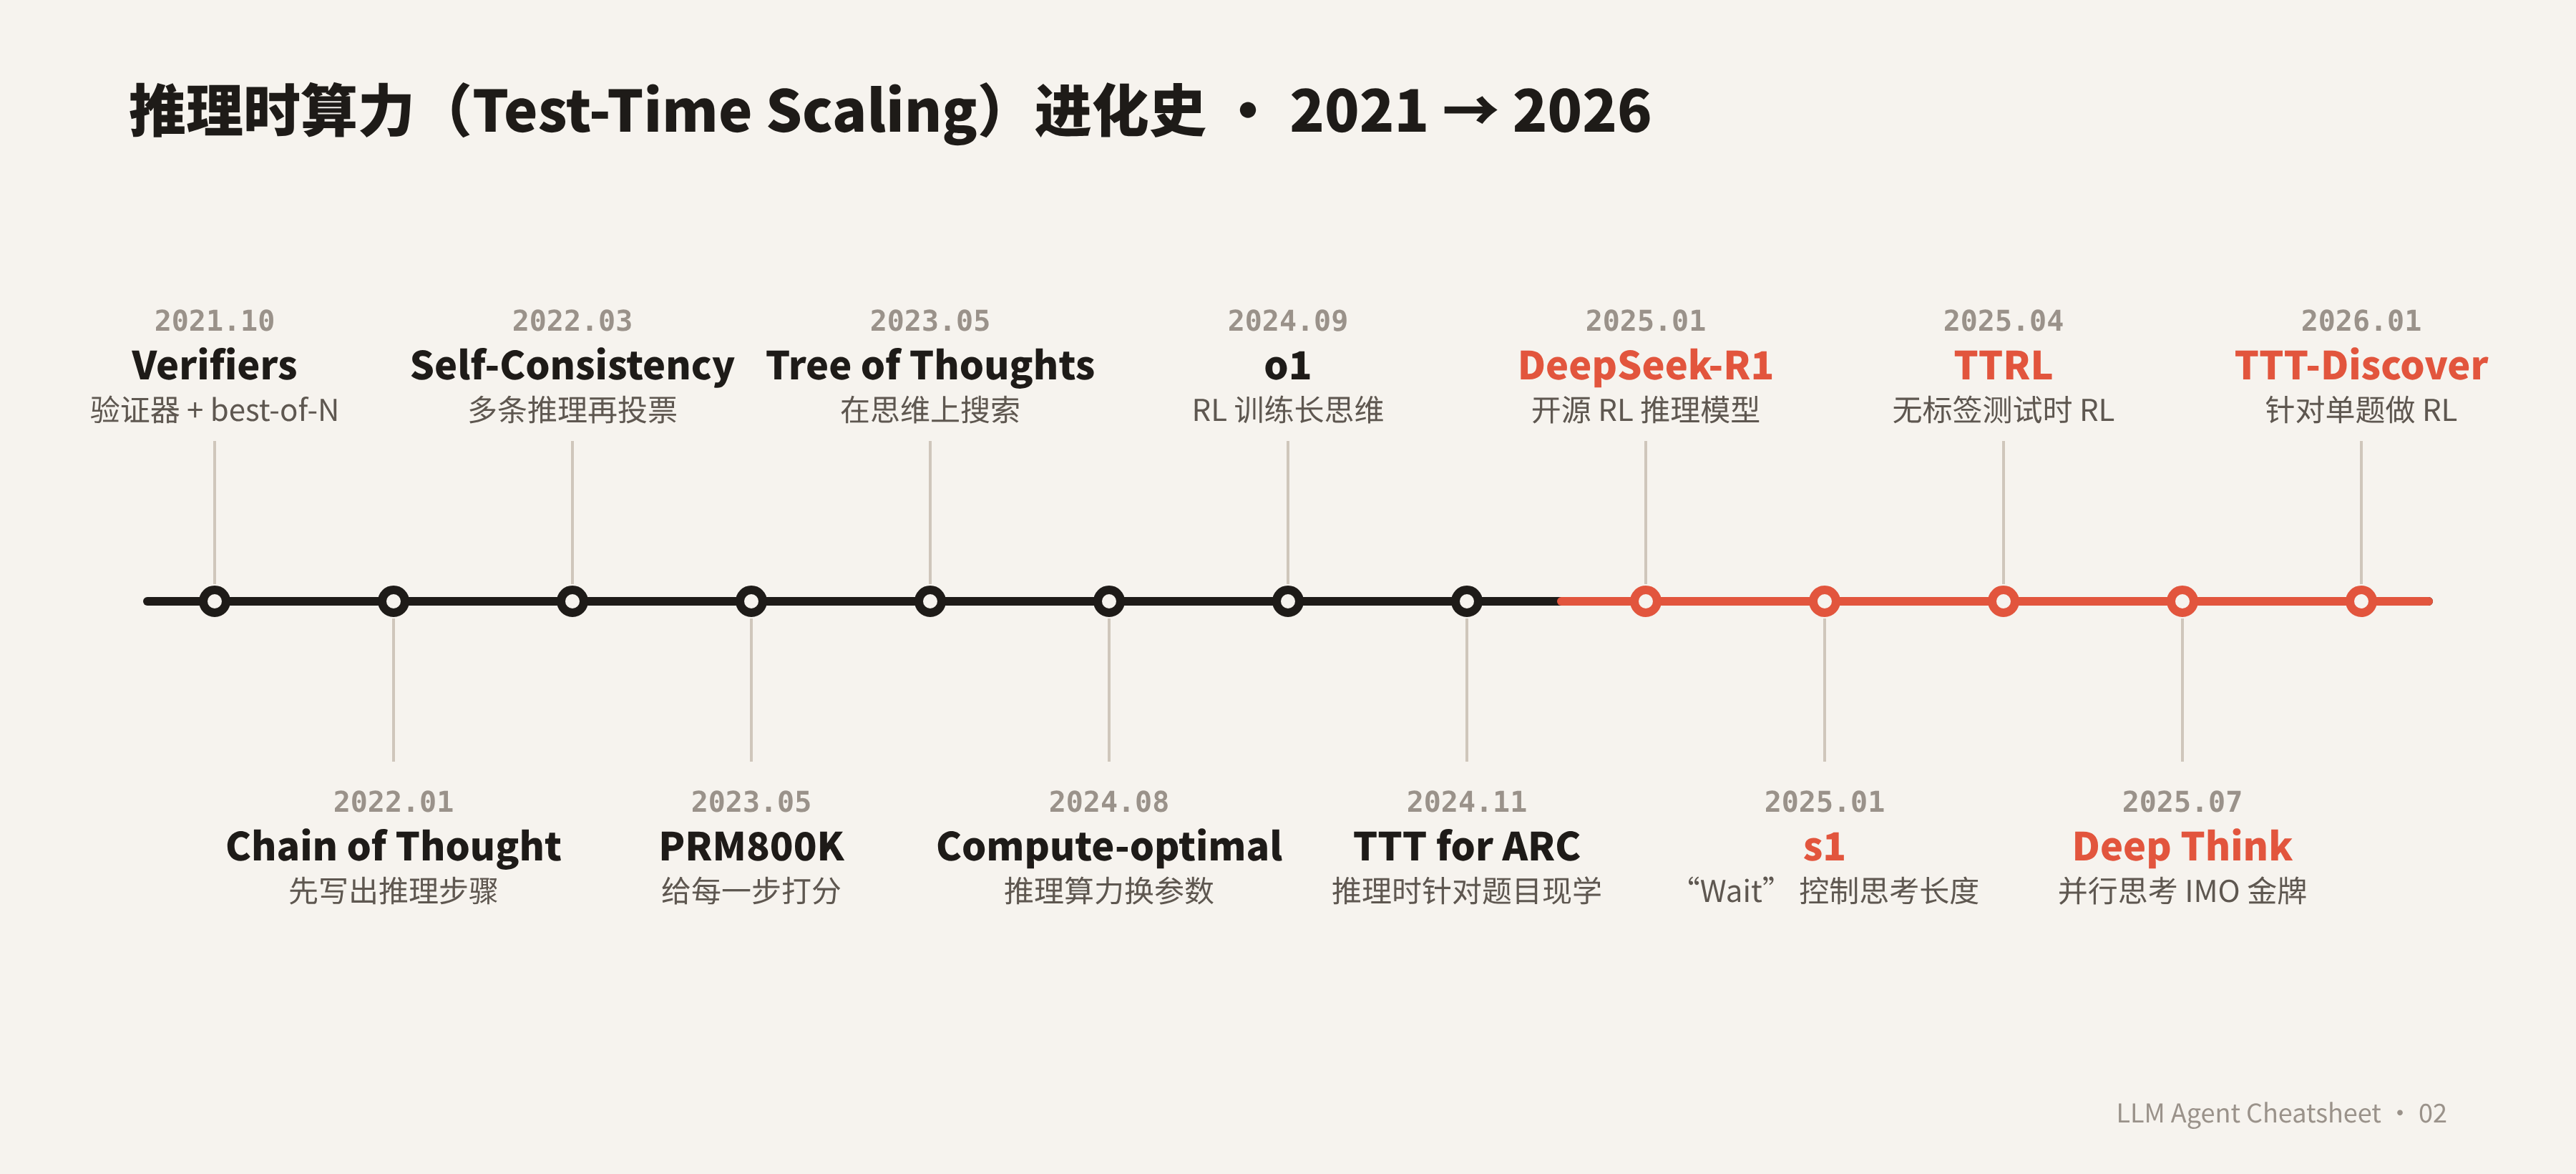
\includegraphics[width=\linewidth]{timeline_zh.png}
\end{tbox}
\end{minipage}\hfill
\begin{minipage}[t]{0.435\linewidth}\vspace{0pt}
\begin{tbox}[title={速查：我的场景该用哪种？}]{cpurple}\small
\textbf{答案能精确比对、没验证器} → 自一致性；开放式输出用 USC\\
\textbf{有可执行测试 / 证明检查} → 大量采样 + 过滤（AlphaCode、Monkeys）\\
\textbf{多步推理、能给步骤打分} → PRM + beam search；没人工标签用 Math-Shepherd / PAV\\
\textbf{预算有限、难度不一} → compute-optimal 分配（Snell）、自适应思考\\
\textbf{要训练推理模型} → 规则奖励 + GRPO（R1），控制长度用 L1 / s1\\
\textbf{分布外、每题有示例} → 测试时训练（TTT-ARC）；无标签用 TTRL\\[1pt]
{\scriptsize\color{cgray}笔者整理的方法路由，不是性能排名。}
\end{tbox}
\begin{tbox}[title={入门必读 6 篇（按顺序）}]{cteal}\small
\begin{tabularx}{\linewidth}{@{}l l Y@{}}
1 & \textbf{Self-Consistency} \ax{2203.11171} & 最简单的并行 scaling\\
2 & \textbf{Let's Verify} \ax{2305.20050} & 过程奖励 vs 结果奖励\\
3 & \textbf{Snell et al.} \ax{2408.03314} & 推理算力怎么换参数\\
4 & \textbf{DeepSeek-R1} \ax{2501.12948} & 只用 RL 训练长思维\\
5 & \textbf{s1} \ax{2501.19393} & 1,000 条数据 + “Wait”\\
6 & \textbf{TTT for ARC} \ax{2411.07279} & 推理时现学\\
\end{tabularx}
\textbf{综述}：What, How, Where, and How Well?（\ax{2503.24235}）· From System 1 to System 2（\ax{2502.17419}）· Stop Overthinking（\ax{2503.16419}）· Trust but Verify（\ax{2508.16665}）
\end{tbox}
\end{minipage}

\vspace{2pt}
\begin{minipage}[t]{0.625\linewidth}\vspace{0pt}
\begin{tbox}[title={自测：看完应该能回答（16 问）}]{cpurple}\normalsize\linespread{1.08}\selectfont
\begin{multicols}{2}
\textbf{Q1} 自一致性和 best-of-N 的区别？\\
前者不需要验证器、只对最终答案投票；后者用验证器打分挑最高的。\\[1pt]
\textbf{Q2} 为什么投票会饱和，甚至越投越差？\\
难题上错误答案可能占多数，样本越多越稳定地选中它。\\[1pt]
\textbf{Q3} 覆盖率（pass@$k$）和实际准确率差在哪？\\
覆盖率假设有 oracle 知道哪个对；实际要靠投票或验证器挑，常在几百个样本后饱和。\\[1pt]
\textbf{Q4} PRM 怎么给整条解打分？\\
各步正确概率相乘（Let's Verify），也有取最小值的做法。\\[1pt]
\textbf{Q5} Math-Shepherd 怎么不用人工标步骤？\\
从该步往后续写 8 次，看能否到达正确答案（hard / soft 两种标签）。\\[1pt]
\textbf{Q6} “compute-optimal” 指什么？\\
按题目难度选推理策略，比 best-of-N 省 4× 以上；小模型 + 推理算力只在中等难度题上胜过大模型。\\[1pt]
\textbf{Q7} 推理 FLOPs 和训练 FLOPs 怎么比？\\
预训练约 $6ND_{\text{pre}}$，推理约 $2ND_{\text{inf}}$；推理次数多时，大模型的推理成本也很高。\\[1pt]
\textbf{Q8} R1-Zero 为什么不用 PRM？\\
神经奖励模型在大规模 RL 中容易被钻空子；规则奖励（答案对错 + 格式）更稳。\\[1pt]
\textbf{Q9} GRPO 和 PPO 的主要区别？\\
用组内归一化的奖励当优势，去掉了价值网络。\\[1pt]
\textbf{Q10} s1 的 budget forcing 怎么做？\\
想停时抑制结束标记、追加 “Wait”；到上限就强制给出答案。\\[1pt]
\textbf{Q11} 过度思考和思考不足分别指什么？\\
简单题写太多 token；难题频繁换思路、每条都没想完。\\[1pt]
\textbf{Q12} 潜空间推理的代价？\\
思考过程不可读、难以监控；数学文字题上还不如显式 CoT。\\[1pt]
\textbf{Q13} TTT 和上下文学习（ICL）的区别？\\
TTT 更新权重，ICL 只用上下文；TTT 层把隐藏状态做成权重，统一了两者。\\[1pt]
\textbf{Q14} TTRL 的奖励从哪来？风险是？\\
多数投票的伪标签；如果初始多数投票就错，会强化错误答案。\\[1pt]
\textbf{Q15} “RL 没有扩展能力边界”的证据和反方？\\
大 $k$ 时基座 pass@$k$ 更高（2504.13837）；ProRL 认为足够长的 RL 能扩展。\\[1pt]
\textbf{Q16} “想得越久越差”的例子？\\
带干扰项的任务（Inverse Scaling）；高复杂度谜题的准确率崩溃（Illusion of Thinking，有争议）。
\end{multicols}
\end{tbox}
\end{minipage}\hfill
\begin{minipage}[t]{0.365\linewidth}\vspace{0pt}
\begin{tbox}[title={关键数字速记}]{cred}\normalsize\renewcommand{\arraystretch}{1.1}
\begin{tabularx}{\linewidth}{@{}l Y@{}}
\toprule
Jones 2021 & 训练 10× ≈ 推理 15×\\
GSM8K 验证器 & 6B + 验证器 ≈ 30× 模型\\
CoT & PaLM GSM8K 17.9 → 56.9\\
Self-Consistency & GSM8K +17.9（40 条）\\
PRM800K & PRM 78.2 / ORM 72.4 / 投票 69.6\\
ToT & 24 点 4\% → 74\%\\
Monkeys & SWE-bench Lite 15.9 → 56\%\\
Snell & >4× 效率；胜 14× 大模型\\
o1 & AIME 74 / 83 / 93\%\\
R1-Zero & AIME 15.6 → 71.0（投票 86.7）\\
s1 & 1K 数据；AIME 50.0 → 56.7\\
过度思考 & 2+3 多用 1,953\% token\\
TTT-ARC & 53\%；集成 61.9\%\\
TTRL & AIME pass@1 约 +211\%\\
Claude 4 并行 & SWE-bench 72.5 → 79.4\\
Deep Think & IMO 2025 35/42\\
DeepConf & token 最多 −84.7\%\\
Gemini 3 DT & ARC-AGI-2 84.6\%（2026-02）\\
Spurious Rewards & 随机奖励 +21.4\\
\bottomrule
\end{tabularx}
\end{tbox}
\end{minipage}

\vfill
{\scriptsize\color{cgray}日期为首次公开月份（arXiv v1 或官方发布）；机构为第一作者主要单位；数字取自原文主结果，不同设置下可能不同。完整中英双语版与全部链接：GitHub \texttt{EvenEureka/llm-agent-cheatsheet}。发现错误欢迎指出。}
\end{document}
